\documentclass[11pt]{article}
\usepackage[utf8]{inputenc}
%\usepackage{fullpage}
\usepackage[margin=25mm]{geometry}
%\renewcommand{\baselinestretch}{1.5} 

%Examples
\usepackage{linguex}

%Tables
\usepackage{multirow}
\usepackage[table]{xcolor}
\definecolor{blue}{HTML}{4E60F0}
\usepackage{colortbl}
\usepackage{array}

%Math
\usepackage{amssymb, stmaryrd}
\usepackage[fleqn]{amsmath}

%Graphics
\usepackage{graphicx}
\graphicspath{{./fig/}}
\usepackage{subcaption}
\usepackage{tikz}
\usetikzlibrary{matrix,positioning}

%Comments
%MORA
\newcommand{\changeMM}[2]{{\leavevmode\color{gray}{\scriptsize\st{#1}}~\color{green}#2}}
\newcommand{\nbMM}[1]{{\leavevmode\color{green}{\scriptsize#1}}}
\newcommand{\addMM}[1]{{\leavevmode\color{green}#1}}

%EWAN
%\newcommand{\changeED}[2]{{\leavevmode\color{gray}{\scriptsize\st{#1}}~\color{red}#2}}
\newcommand{\changeED}[1]{{\textcolor{red}{#1}}}
\newcommand{\nbED}[1]{{\leavevmode\color{red}{\scriptsize#1}}}
\newcommand{\addED}[1]{{\leavevmode\color{red}#1}}

%EMMANUEL
%\newcommand{\changeEC}[2]{{\leavevmode\color{green}{\scriptsize\st{#1}}~\color{green}#2}}
\newcommand{\changeEC}[2]{{\footnotesize\textcolor{gray}{#1}}\textcolor{blue}{#2}}
\newcommand{\nbEC}[1]{{\leavevmode\color{blue}{\scriptsize#1}}}
\newcommand{\addEC}[1]{{\leavevmode\color{blue}#1}}


%References and bibliography
\usepackage{hyperref}
\usepackage[noabbrev,capitalise,nameinlink]{cleveref}
\hypersetup{colorlinks={true},linkcolor={blue},citecolor=magenta}
%\usepackage{natbib}

\usepackage[natbibapa]{apacite}
\bibliographystyle{apacite}

%Line numbers
%\usepackage{lineno}
%\linenumbers




\title{Mouse tracking as a window into decision making}
\author{Mora Maldonado, Ewan Dunbar \& Emmanuel Chemla}

\begin{document}

\maketitle

\begin{abstract}
Mouse tracking promises to be an efficient method to investigate the dynamics of cognitive processes: it is easier to deploy than eye-tracking, and yet it is in principle much more fine-grained than looking at response times.
We investigate its claimed benefits directly, asking how features of decision processes, and notably decision changes, may be captured in mouse movements. 
We ran two experiments, one in which we explicitly manipulate whether our stimuli trigger a flip in decision, and one in which we replicate more ecological, classical mouse tracking results on linguistic negation \citep{Dale2011}.
We conclude, first, that spatial information (mouse path) is more important than temporal information (speed and acceleration) for detecting decision changes, and we offer a comparison of the sensitivity of various typical measures used in analyses of mouse tracking (area under the trajectory, direction-flips, and others). We do so using an `optimal' analysis of our data (a linear discriminant analysis) explicitly trained to classify trajectories), and see what type of data (position, speed, acceleration) it capitalizes on. We quantify how its results compare with those based on more standard measures.

\end{abstract}




\section{Introduction}

In the past ten years, mouse tracking has become a popular method for studying the dynamics of cognitive processes in different domains, ranging from phonetic competition \citep{Spivey2005,cranford2017mouse}, and syntactic, semantic and pragmatic processing \citep[among others]{Farmer2007, Dale2011, tomlinson2013possibly,xiao2014semantic,sauerland2015tracking,xiao2017role}, to social cognition \citep{Freeman2010,Freeman2011,freeman2016more}.
While response times can reveal whether a decision process is fast or slow \citep{donders1969speed}, and analyses of response time distributions can give insight into how the decision process unfolds \citep[among others]{usher2001time,ratcliff2008diffusion}, mouse movements promise a more direct window onto the dynamics of cognitive processes, under the assumption that motor responses are planned and executed in parallel to the decisions they reflect \citep{song2006role,Song2009,Freeman2010,spivey2006continuous,Hehman2014}.

Concretely, if a response is entered by clicking on a button, one may measure the time needed to click on that button and use it as a reflection for the complexity of the decision, roughly. But depending on whether participants are decided from the start, hesitate, or undergo a radical change of decision, the path to that button may take different trajectories (see \Cref{fig:scheme.traj}, \citealp{Wojnowicz2009}). %
Accordingly, researchers have studied the shape and dynamics of mouse paths to document aspects of numerous types of decision processes. Dale and Duran's (\citeyear{Dale2011}) approach to negation processing is an example of this.   
Linguistic negation has been traditionally understood as an operator that reverses sentence truth conditions, inducing an extra ``step,'' or ``mental operation,'' in online processing (\citealp{wason1965contexts,wason1972psychology}; see review in \citealp{Tian2016}). %
Dale and Duran tracked mouse trajectories as participants performed a truth-value judgment task, where they had to verify the truth of general statements such as \textit{Cars have (no) wings}.
%
The authors found that mouse trajectories gave rise to more shifts towards the alternative response when evaluating negative than affirmative true sentences. This was interpreted as evidence for a ``two-step'' processing of negation, where truth conditions for the positive content are first derived and negated only as a second step.% 
%
\footnote{Several studies have suggested that the positive argument plays an important role in negation processing \citep[among others]{kaup2007experiential,ludtke2008event}.  
This pattern of results, however, depends on the amount of contextual support given for the sentence: ``two-step'' negation processing seems to occur specifically for sentences presented out-of-the-blue, whereas no difference between negative and positive sentences arises when the right contextual support is provided \citep{nieuwland2008truth,tian2010we}. How to explain this pattern of results has been at the center of the debate in the negation processing literature (see \citealp{Tian2016} for review). We will not explore this here.}
To do so, one can extract several measures from the mouse paths (e.g., maximal deviation point, number of direction changes, etc.) and argue that the deviation of these measures from what they would be for an optimal, straight trajectory reflects the relevant decision change.

%\changeEC{The impact of experimental manipulations on the shape of trajectories has thus been taken as evidence for underlying decision patterns in many domains. This association, however, has never been explicitly tested and there surely is not a dictionary that could help us translate between decision processes (decision changes, hesitations, etc.) and mouse paths.}{}


\begin{figure}[h]
\centering
\includegraphics[width=0.8\textwidth]{trajectories.jpeg}
\caption{\textbf{Shape of trajectories underlying distinct decision processes.} One single cognitive process is expected to be mapped onto one smooth trajectory (blue line), whereas a change of mind would be reflected by a two-step path (red line). Intermediate cases are represented in gray.} \label{fig:scheme.traj}
\end{figure}

Our goal is to explicitly document this method and the connection between cognition (decision making) and action (mouse trajectories): What in a decision process is reflected in mouse movements---decision changes, hesitations, or other properties?--- and how ---in changes in acceleration, changes in direction, or other aspects of the trajectory? %(acceleration picks, changes of directions, etc.)?
%One could imagine a situation where two different trajectory shapes do not correspond to two different decision mechanisms, but to a single one (due to uncertainty, noise, etc.). Differences in trajectories can therefore underlie something other than decision shift. 
We will tackle this question by asking what features of mouse trajectories distinguish \emph{straightforward} decisions, based on a single initial commitment, and \emph{switched} decisions, which involve a change of mind in the course of the process.%
 

First, we present a validation experiment where we directly manipulate whether the stimuli trigger a flip in what the appropriate response is in the course of a trial.
%decision, and show qualitatively
We show that the mouse paths do indeed reflect these changes (\Cref{section:validation}). 
An analysis of this data using linear discriminant analysis (henceforth, LDA), confirms that the two types of decision, straightforward 
and switched, can be distinguished objectively (\Cref{section:LDA}). 
%The data from this validation experiment (that is, two groups of `quasi-decisions') is then fed to a \emph{Linear Discriminant Analysis} (henceforth, LDA), trained to classify trajectories depending on the underlying type of decision, straightforward or switched (\Cref{section:LDA}). 
We then compare the performance of the LDA classifier to other traditionally used mouse tracking measures (\Cref{section:other-mt}). 
Finally, the LDA classifier trained on the validation data is further tested with new, more ``ecological'' data, obtained from a replication of Dale and Duran's (\citeyear{Dale2011}) experiment on the processing of negation mentioned above (\Cref{section:replication}). If there is a change of decision triggered by negation, trajectories corresponding to negative trials should be classified together with trajectories underlying changes of decision in the validation experiment. 

Data and code for all the analyses developed in this paper are provided at \url{https://osf.io/rbx3m/?view_only=7d557aa8931c4a0886e7ce2442a77895}.

\section{Validation Experiment: presentation and qualitative analysis}
\label{section:validation}

Participants were asked to perform a two-alternative forced choice task. Each trial was triggered by clicking on a start button at the bottom of the screen. A frame surrounding the screen would then appear and the participants' task was to indicate whether the frame was blue or red by clicking on the appropriate ``blue" or ``red" buttons at the top left or top right of the screen, respectively. %Mouse-movements were recorded between during each trial. Responses were considered accurate if they described the color at the moment of the click. 
On most trials, the color of the frame remained stable throughout the trials, but in crucial cases it changed during the trial.
In the first case, the initial choice was the correct response (\textit{straightforward} trials. In the second case, participants were forced to change their answer (\textit{switched} trials). The switched trials are meant to mimic natural decision changes. We take these to be a reasonable stand-in for changes of decision, even though there are obvious differences: in natural changes of decision, alternative responses are weighted as the pieces of information are integrated, whereas in our experiment the sensory information changes in time.
We return to the question of how ecological these decisions are in \Cref{section:replication}.
The procedure is illustrated in \Cref{fig:procedure.example}. 


\begin{figure}[h]
\centering
\includegraphics[scale=.5]{procedure.pdf}
\caption{\textbf{Procedure in Validation Experiment.} Subjects were instructed to click the ``start'' button in order to see the colored frame. Response boxes were on the top left or top right. Depending on the trial condition, the frame color either did, or did not, change (once) during the trial.} \label{fig:procedure.example}
\end{figure}

\subsection{Participants} We recruited 54 participants (F=27) using Amazon Mechanical Turk. Two subjects were excluded from the analyses because they did not use a mouse to perform the experiment. All of them were compensated with 0.5 USD for their participation, which took approximately 5 minutes. 

\subsection{Design}
Each trial instantiated one of two possible \textsc{Decision pattern}s. In \textit{straightforward} trials, the frame color remained stable, and the decision made at the beginning of the trial did not need to be revised. In \textit{switched} trials, the color switched once (from red to blue or from blue to red) during the trial, forcing a revision of the initial choice. 
The change on \textit{switched} trials was triggered by the cursor reaching a certain position on the \textit{y}-axis, which could be at various relative heights (\textsc{point of change}: early, at 40\% of the screen, middle, at 70\%, or late, at 90\%). 
%The \textsc{Frame color} at the response point was also controlled: it could be red (right button) or blue (left button).    
The design is schematized in \Cref{tab:design.validation}. 


\begin{table}[!h]
\centering
\begin{tabular}{cc>{\centering\arraybackslash}c}
\textsc{Decision Pattern}& \textsc{Frame color}& \textsc{Point of change}\\
\hline
\noindent\parbox[c]{9em}{Straightforward} & 
	\begin{tabular}{c}Blue\\Red\end{tabular} &  \emph{never}\\
\hline

  \noindent\parbox[c]{9em}{Switched} & 
  \begin{tabular}{ccc}
  Blue & $\rightarrow$ & Red\\
  Red & $\rightarrow$ & Blue\\
  \end{tabular} &
  \begin{tabular}{cc}
  early & (y=40\%)\\
  middle & (y=70\%)\\
  late & (y=90\%)\\
  \end{tabular}   
\end{tabular}

\caption{\textbf{Design in Validation Experiment}}
\label{tab:design.validation}
\end{table}

To prevent participants from developing a strategy whereby they simply drag the cursor along the center line rather than moving the mouse toward their current choice of answer, the proportion of trials was adjusted so that there were a majority of 64 straightforward trials (32 repetitions per frame color), while there was only 24 switched trials (4 repetitions per final frame color and change point). 

\subsection{Interface}

The web interface was programmed using JavaScript. Mouse movements triggered the extraction of $(x,y)$-pixel coordinates (there was thus no constant sample rate).
% The coordinates were proportional to the window of the participant's browser, forming a rectangle. 
%(height at 100 percent; width at 120 percent of the height). 
Three buttons were displayed during the experiment (``start'' and response buttons). The ``start'' button was placed at the bottom center of the screen. The two response boxes were located at the top left (``blue'') and top right (``red'') corners. 
On each trial, between start-clicks and response-clicks, mouse movements triggered the recording of the $(x,y)$-pixel coordinates of the cursor together with the time. 


\subsection{Data treatment}
To allow comparisons between participants, the $(x,y)$-coordinates were normalized according to participants' window size: the center of the start button was mapped onto $(0,0)$ point, the ``blue'' button onto $(-1,1)$ and the ``red'' button onto $(1,1)$. 
Variations both in response times and in the sensitivity and sampling rate of our participants' input devices imply that different trials have different numbers of $(x,y)$ positions per trial, making comparisons difficult. %Moreover, in our design, positions are extracted based on mouse movements, and devices with different sensibility can influence the number of samples taken during the trial. 
We therefore normalized the time course into 101 proportional time steps by linear interpolation. That is, we reduced all time points to 101 equally distant time steps, including the first and the last positions.

\subsection{Overall performance}
Inaccurate responses (4\% of the data) were removed from the analyses. 
Mean trajectories for each \textsc{decision pattern} and \textsc{point of change} are illustrated in \Cref{fig:mean.trajectories.calibration}. 
%Temporal information about changes in the $x$ coordinate is provided in the appendix (Figure X). 
These trajectories suggest that participants made a decision as soon as they were presented with the color frame, and revised this decision if needed. When they were forced to change their choice, this switch was reflected in mouse trajectories. 

\begin{figure}
\centering
\includegraphics[width=\textwidth]{mean-trajectories-validation.png}
\caption{\textbf{Mean trajectories for different decision patterns in the validation experiment.} Error bars represent the standard error of $x$-coordinates.}\label{fig:mean.trajectories.calibration}
\end{figure}

\section{Validation Experiment: Classifying decision processes with LDA}
\label{section:LDA}
Different decisions (that is, \textsc{Decision pattern}s) have a different impact on mouse trajectories (\Cref{fig:mean.trajectories.calibration}). To identify the features characteristic of each class (\textit{switched} vs.\ \textit{straightforward}), we use a linear discriminant analysis for classification. 

\subsection{Description of LDA classifier}
The LDA is a supervised algorithm that finds a linear function of the predictors onto a single real number, such that zero represents the midpoint between the two classes to be learned, and the separation between the two classes is maximal. This linear combination of predictors can thus be used to form a decision rule to classify objects of one class (negative) or the other (positive).
 
The two classes here were the multi-dimensional data coming from \emph{switched} and \emph{straightforward} trials. The dimensions taken into account were: all the \textit{x,y} coordinates, the Euclidean-distance based velocity and the Euclidean-distance based acceleration (both of which are non-linear with respect to the original $(x,y)$ coordinates). The coordinates provide absolute spatiotemporal information about where the cursor was at what point, and velocity and acceleration provide information about how it arrived there.
To avoid collinearity (which causes problems for LDA), we applied a principal component analysis (PCA) to identify 13 principal components for these predictors, and fitted and applied the LDA to these principal components.
We thus obtained an \emph{LDA measure} for each trial, the single number giving the position of the trial on the LDA classification axis.
The procedure is schematized in \Cref{fig:diagram}.

\begin{figure}
\centering
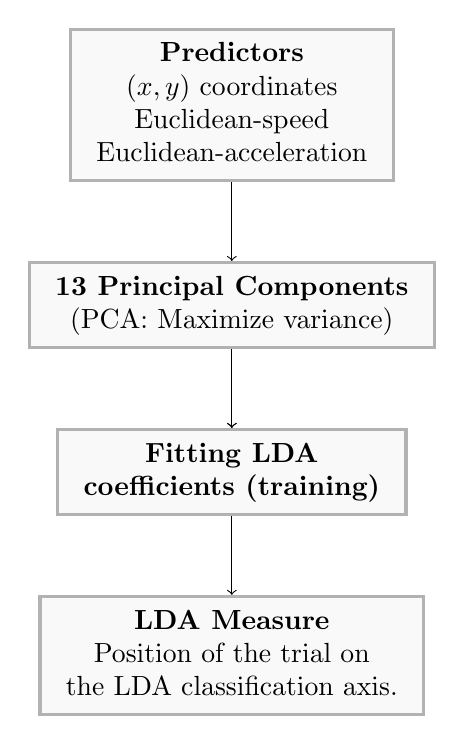
\begin{tikzpicture}[
squarednode/.style={rectangle, draw=gray!60, fill=gray!5, very thick, minimum size=5mm},
squarednode2/.style={rectangle, draw=red!60, fill=red!5, very thick, minimum size=5mm},
]

%Nodes
\node[squarednode]      (pca)                              {\begin{tabular}{c} \textbf{13 Principal Components} \\ (PCA: Maximize variance)\end{tabular}};

\node[squarednode]        (pred)       [above=of pca] {\begin{tabular}{c} \textbf{Predictors} \\ $(x,y)$ coordinates \\ Euclidean-speed \\ Euclidean-acceleration \end{tabular}};
  \node[squarednode]      (lda)       [below= 1cm of pca] {\begin{tabular}{c} \textbf{Fitting LDA}\\\textbf{coefficients (training)}\end{tabular}};
  \node[squarednode]        (ldameasure)       [below=1cm of lda] {\begin{tabular}{c} \textbf{LDA Measure}\\ Position of the trial on \\ the LDA classification axis. \end{tabular}};
 
%Lines
\draw[->] (pred.south) -- (pca.north);
\draw[->] (pca.south) -- (lda.north);
\draw[->] (lda.south) -- (ldameasure.north);
\draw[->] (pca.south)  -- (lda.north);

\end{tikzpicture}
\caption{\textbf{Diagram of classification procedure.}}\label{fig:diagram}

\end{figure}

\subsection{Performance of the LDA classifier}
\Cref{DIST:LDA} illustrates the result of applying the procedure in \Cref{fig:diagram} to the trajectories. 
To evaluate the overall performance of the classifier, we calculated the area under the ROC curve (AUC), a standard method for evaluating classifiers \citep{Hastie}. Intuitively, the AUC gives the degree to which the histograms resulting from the classifier's continuous output (for example, \Cref{DIST:LDA}) are non-overlapping in the correct direction (in this case, \textit{switched} more systematically in the positive direction on the classification axis than \textit{straightforward}). 


\begin{figure}
\centering
\includegraphics[width=.8\textwidth]{lda_distribution_calibration.png}
\caption{\textbf{Distribution and mean LDA-based measure for each class.} Classifier performance when applied to the whole validation data set. Error bars represent the mean standard error.} \label{DIST:LDA}
\end{figure}

To properly evaluate the classifier's performance at separating trials following the distribution in the experiments, the AUC measure was cross-validated. That is, calibration data were partitioned into 10 bins that kept the proportion of \textit{straightforward} and \textit{switched} trajectories constant (75/25 proportion). For each bin, we took the complementary set of data (the remaining 90\%) to train the classifier. The data contained in the bin were used as a test set to diagnose the classifier performance. We thus obtained one AUC score for each of the ten test bins. The performance of the LDA classifier was compared to a baseline, equivalent to the worst possible outcome, and a topline, which was what we would expect from a LDA under the best possible conditions. 
For the baseline, we used a random classifier that assigned labels by sampling from a beta distribution centered at the probability of straightforward trials; the topline was computed by testing and training the original LDA classifier on the same set of data. 
The mean AUC values for the LDA, the baseline and the topline in each bin are given in \Cref{DIST:AUC}a. 

To assess whether the performance of the LDA classifier was statistically different from baseline (or topline) performance, we tested the groups of ten scores with regard to how likely it would be to obtain the attested differences in scores under the null hypothesis that the LDA classifier performance was the same as baseline (or topline) performance.   
The difference in the mean AUC between each of these two pairs of classifiers was calculated as a test statistic. The sampling distribution under the null hypothesis was estimated by randomly shuffling the labels indicating which classifier the score came from.

In \Cref{table:comparisons.permutation.1}a, we report the results of performing a one-tailed test on the mean AUC differences. As expected, our original LDA is significantly better than a random classifier at categorizing trajectories into \emph{straightforward} and \emph{switched.} Conversely, there is no significant difference between the performance of our LDA and the topline; the classifier's performance is not significantly different from the best an LDA could possibly give on this data. 

\begin{figure}[h]
\centering
\includegraphics[width=\textwidth]{auc_calibration_1.png}
\caption{\textbf{Mean Area Under the ROC Curve values obtained from cross-validation.} A. Cross-validation on 10 bins for original LDA, baseline and topline. B. Comparison with values obtained for five additional classifiers obtained by subsetting the original set of predictors.} \label{DIST:AUC}
\end{figure}


\begin{table}[h]
\centering
{\footnotesize
\begin{tabular}{p{1.6cm}>{\columncolor[gray]{0.8}}p{1.5cm}cc|p{1cm}cccc}

 \multicolumn{2}{c}{ } &  \multicolumn{2}{c}{(a)} & \multicolumn{4}{c}{(b)}\\
\hline
& \centering \textsc{Original LDA}& \multirow{2}{*}{\centering \textsc{Baseline}} & \multirow{2}{1.1cm}{\textsc{Topline}} &\multicolumn{5}{c}{\textsc{LDA with different predictors}}\\
\cline{5-9}
& \centering (coords, speed, acc) &  & & \centering coords, vel & vel, acc & coords & vel & acc \\[0.5cm]

\hline
\centering \textbf{AUC (mean)} & \centering .87& .52 & .87 &\centering .87 & .83 & .87 & .82 & .67 \\[0.5cm]

\hline
\centering \textbf{Mean \\ Difference} & \centering -- & .35 & -.002 &\centering -.0004 &  .04 & -.006 & .04 & .2 \\[0.5cm]



\hline
\centering \textbf{$p$ value} & \centering  --  &  $<$.001 & 0.58 & \centering .5 & $<$.001 & .68 & $<$.001 & $<$.001 \\
%& .72 & $<$.001 \\
\hline
\end{tabular}}
\caption{\textbf{Cross-validation results for the LDA classifier.} The performance of the LDA was compared to the one of (a) baseline and topline classifiers and (b) LDA classifiers with different predictors.}
\label{table:comparisons.permutation.1}
\end{table}

\subsection{Meaningful features and optimal predictors}
Our original LDA classifier takes as predictors both absolute and relative spatio-temporal features (coordinates, speed, and acceleration).
Some of these features, however, might not be relevant for the classification. 
By comparing classifiers trained with different predictors, we gather information about which features of mouse trajectories are most relevant to decision processes. 

We trained five additional LDA classifiers obtained by subsetting the three original LDA predictors. If both absolute and relative features are required to predict the decision type, we would expect our ``full'' original LDA classifier to be better than any other classifier that takes only a subset of these original predictors. 
The performance of these additional classifiers was diagnosed in the same way as before, by computing the AUC for each of the 10 test bins. \Cref{DIST:AUC}b illustrates the mean AUC values for each of these classifiers, together with the original LDA, the baseline and the topline. 
Pairwise comparisons with the original LDA were done by testing whether the observed mean differences would be expected under the null hypothesis of no difference in performance between classifiers. \Cref{table:comparisons.permutation.1}b summarises the comparisons between each of these classifiers and our original LDA. 	

The original LDA does not significantly differ from other LDA classifiers that contain the coordinates among their predictors, suggesting that the distinction between \emph{straightforward} and \emph{switched} decisions might be solely explained by the information contained in the $(x,y)$ coordinates. 
Conversely, the original LDA is significantly better than classifiers that use only speed and acceleration as predictors. These comparisons therefore reveal that, for classifying our validation data, absolute spatio-temporal features ($(x,y)$ coordinates) are generally better predictors than relative features (speed and acceleration). That is, it seems to be more relevant to know where the mouse pointer was at a given time than to know how it got there. 

We caution that effects of \emph{true} decisions, rather than the simulated decisions tested here, may indeed have an impact on speed and acceleration. It has been suggested that speed and acceleration components can capture the level of commitment towards the response, such that a change of decision (\textit{swiched} trajectories) might have associated with it a specific speed/acceleration pattern \citep{Hehman2014}. This is not visible, however, in our data.


\section{Validation Experiment: LDA \emph{versus} traditional mouse tracking analyses}
\label{section:other-mt}
The LDA classifier derives a solution to the problem of separating two kinds of mouse trajectories that is in a certain sense optimal. Previous studies have used alternative techniques to analyze mouse trajectories. In what follows, we  compare the performance of our LDA to other measures commonly used in mouse tracking studies. We focus on measures that assess the spatial disorder in trajectories, typically taken to be indicative of unpredictability and complexity in response dynamics \citep{Hehman2014}.

Two of the most commonly used methods of mouse tracking \textbf{spatial analysis} are the \textit{Area under the trajectory} and the \textit{Maximal deviation} (henceforth, AUT and MD respectively) (see \citealp{Freeman2010}).
The AUT is the geometric area between the observed trajectory and an idealized straight-line trajectory drawn from the start to the end points, whereas the MD is the point that maximizes the perpendicular distance between this ideal trajectory and the observed path
(\Cref{fig:traditional-measures}). For both measures, higher values are associated with higher trajectory deviation towards the alternative; values close to or below zero suggest a trajectory close to ideal. 
Another frequently used measure counts the number of times a trajectory crosses the $x-$axis (horizontal flips, \citealp{Dale2011}, as illustrated in \Cref{fig:traditional-measures}).




\begin{figure}[h]
\centering
\begin{subfigure}[b]{0.3\textwidth}
\includegraphics[width=\textwidth]{AUC.pdf}
\caption{Area Under the Trajectory}
\end{subfigure}
%
\begin{subfigure}[b]{0.3\textwidth}
\includegraphics[width=\textwidth]{MD.pdf}
\caption{Maximal Deviation}
\end{subfigure}
%
\begin{subfigure}[b]{0.3\textwidth}
\includegraphics[width=\textwidth]{MaxRatio.jpeg}
\caption{Maximal Log Ratio}
\end{subfigure}
\vspace{.5cm}

\begin{subfigure}[b]{0.45\textwidth}
\caption{X-coordinate Flips}
\centering
\(\sum H[(x_{t} - x_{t-1})(x_{t-1} - x_{t-2})] \)
\end{subfigure}
%
\begin{subfigure}[b]{0.45\textwidth}
\caption{Acceleration flips}
\centering
\((\sum H[( a_{t} - a_{t-1})( a_{t-1} - a_{t-2})])-1 \)

\end{subfigure}

\caption{\textbf{Description of commonly used mouse tracking measures.}}
\label{fig:traditional-measures}

\end{figure}



While all these measures aim to evaluate the degree of complexity of the path, they may fail to distinguish paths straight to the correct answer from ``two step'' (deviation to the alternative) and from ``uncertain'' (centered on the middle of the screen) trajectories.%
%
\footnote{A late medium-size deviation towards the alternative might underlie a ``two-step'' decision, whereas an early, but large, deviation towards the alternative might very well be considered noise. Measures such as the AUT might not be able to make a distinction between these.} 
To assess more directly whether mouse trajectories have a meaningful deviation towards the alternative, the distance to both target and alternative responses should be taken into account. 
For instance, the \textit{ratio of the target distance to the alternative distance} can be calculated for each $(x,y)$ position. While ratio values closer to one suggest a position near the middle, higher values indicate a deviation towards the alternative response. 

AUT, MD, $x$-coordinate flips, and the point that maximizes the log distance ratio (henceforth Maximal Log Ratio)  % Maximal Log Ratio, henceforth) 
were calculated for the validation data. 
Following Dale and Duran (\citeyear{Dale2011}, and other studies on error corrections), we also analyzed the \emph{acceleration component} (AC) as a function of the number of changes in acceleration.
% \addMM{(NB: This is not the same as computing the number of times the acceleration changes direction, going from positive to negative acceleration, as D\&D claim)}. 
Since stronger competition between alternative responses is typically translated into steeper acceleration peaks, changes in acceleration can be interpreted as decision points \citep{Hehman2014}.   
\Cref{fig:different.measures.validation} illustrates the distribution and mean values for each decision pattern.
%Following the procedure in Dale and Duran (2011), trajectory velocity and acceleration were computed using the distance (in pixels) covered per second over a moving window of six $(x,y)$ pixel coordinates. The number of acceleration flips were calculated on this smoothed acceleration. 

The same cross-validation procedure described in the previous section was used to diagnose the performance of each of these measures.\footnote{Note that these measures do not need training; we simply applied the measure to the same ten test subsets as before to make the results comparable.} The mean AUC values for each of these measures are illustrated in \Cref{DIST:AUC2}. \Cref{table:comparisons.permutation.2} summarizes the result of comparing the LDA performance to each of the alternative measures. 



\begin{figure}
\centering
\begin{subfigure}[b]{0.4\textwidth}
\includegraphics[width=\textwidth]{AUC_calibration.png}
\caption{Area Under the Trajectory}
\end{subfigure}
%
\begin{subfigure}[b]{0.4\textwidth}
\includegraphics[width=\textwidth]{MD_calibration.png}
\caption{Maximal Deviation}
\end{subfigure}

%
\begin{subfigure}[b]{0.4\textwidth}
\includegraphics[width=\textwidth]{MaxRatio_calibration.png}
\caption{Maximal Log Ratio}
\end{subfigure}
%
\begin{subfigure}[b]{0.4\textwidth}
\includegraphics[width=\textwidth]{Xflips_calibration.png}
\caption{X-coordinates Flips}
\end{subfigure}

\begin{subfigure}[b]{0.4\textwidth}
\includegraphics[width=\textwidth]{AC_calibration.png}
\caption{Acceleration Component}
\end{subfigure}

\caption{\textbf{Distribution and means obtained from applying different mouse tracking measures to validation data.} Error bars represent the mean standard error.}
\label{fig:different.measures.validation}

\end{figure}


\begin{figure}
\centering
\includegraphics[width=\textwidth]{auc_calibration_2.png}
\caption{\textbf{Mean Area Under the ROC Curve values obtained from cross-validation.} A. Cross-validation on 10 bins for original LDA, baseline and topline. B. Comparison with values obtained for other commonly used mouse tracking measures.} \label{DIST:AUC}
\label{DIST:AUC2}
\end{figure}

\begin{table}[h]
\centering
{\small
\begin{tabular}{p{1.7cm}>{\columncolor[gray]{0.8}}p{1.5cm}cp{1.4cm}p{1.7cm}p{1.6cm}c}
& \centering \textsc{Original LDA}& \textsc{AUT} & \centering \textsc{MD} & \centering\textsc{Maximal LogRatio} & \centering\textsc{X-Coord. Flips} & \textsc{AC} \\

\hline
\centering \textbf{AUC (mean)} & \centering .87 & .62 &  \centering .81 &  \centering.81 & \centering.73 & .53 \\[0.5cm]
\hline 
\centering \textbf{Mean \\ Difference} & \centering--& .24 & \centering .06 &  \centering.06  & \centering .14 & .34  \\[0.5cm]
\hline
\centering \textbf{$p$ value} &\centering -- & \centering$<$.001&\centering $<$.001&\centering$<$.001&\centering$<$.001&$<$.001\\
\hline
\end{tabular}}
\caption{\textbf{Cross-validation results for the LDA classifier.} The performance of  LDA was compared to each of five commonly used measures in mouse tracking studies.}
\label{table:comparisons.permutation.2}
\end{table}
Overall, these comparisons reveal that the LDA trained on the validation data is significantly better at classifying this type of decisions than other commonly used measures. The difference with the classifier is in all the cases significant. Mean AUC values suggest that MD and the Maximal Log Ratio are better at distinguishing decision processes than the other alternative measures. These two measures are the only ones calculated based on coordinates, and therefore give more importance to spatio-temporal information than the others. 
In other words, the MD and the Maximal Log Ratio are not only sensitive to whether or not there was a deviation from the ideal trajectory (as the other measures), but weight this deviation as a function of the moment at which it occurred, assigning higher values to late deviations.
%In other words, both the MD and the Maximal Log Ratio give different weight to positions depending on the moment when they occurred,\nbEC{not clear} and therefore are more sensitive to the moment at which deviation occurred. 
This information seems to be essential for the classification, as observed in \Cref{section:LDA}. 



Finally, we previously observed that velocity and acceleration were not helpful predictors for the LDA classifier. Indeed, the performance of the Acceleration Component overlaps here with that of the Baseline, suggesting that this type of information is not helpful.


\section{Extension to linguistic data}
\label{section:replication}
So far, we have shown that (i) a rough manipulation of decision making processes has a direct impact on mouse trajectories; (ii) an LDA using absolute temporal information is enough to accurately distinguish these decision patterns; and (iii) this LDA does a better classification than other traditional mouse tracking measures. Can our LDA help characterize more complex decision processes, such as the ones involved in sentence verification tasks? 
%\nbEC{This paragraph is needed, but I don't know how to present it: it is odd on its own as a section, but it is also odd as part of the previous paragraph which is only about (iii). It could be an introduction to the next section, but I fear it won't be salient enough. I am not sure what to do then.}\nbMM{I think it's better as part of the following section}
%How well does our LDA, trained on “quasi-decisions”, classify new trajectories, which underly cognitive processes that might or not correspond to different decision patterns? 
\paragraph{}
To address this question, we test our classifier on data obtained from a replication of Dale and Duran's experiment (\citeyear{Dale2011}).   
%Dale and Duran (\citeyear{Dale2011})
This experiment found differences in the processing of true positive and negative sentences when people performed a truth-value judgment task. These results were interpreted as indicating that negation gives rise to an abrupt shift in cognitive dynamics (an unconscious change of decision). If this is indeed the case, we would expect mouse trajectories corresponding to the verification of negative sentences to pattern with \emph{switched} trajectories from the validation experiment. This pattern of results would provide additional support to the hypothesis that, at least in out-of-the-blue contexts, processing negation does involve two steps, in which the positive value is initially derived and negated only as a second step.
%\footnote{We reiterate that, since the training set is only an approximation of what should happen during an unconscious change of decision, we expect some aspects of the decision processes on sentence-verification data not to be captured by the LDA.}
On the other hand, if negation does not involve a change in decision---or if subjects' behavior in the validation experiment is simply too different from natural changes of decision---then the LDA measure trained on validation data will not reveal systematic differences between positive and negative sentences.


\subsection{Experiment}
Participants had to perform a truth-value judgment task in which they had to decide whether a sentence (for example, \textit{Cars have wheels}) is true or false, based on common world knowledge. Each sentence could either be a negated form or a non-negated form, and could either be a true or a false statement.
Unlike Dale and Duran's experiment, the complete statement was presented in the middle of the screen after participants pressed ``start'' (that is, no self-paced reading). The response buttons appeared at the top left or top right corners of the screen, as in our validation experiment.  
Materials and design are exemplified in \Cref{table:exampleDD}. 

\subsubsection{Participants}
53 English native speakers (F=29) were tested using Amazon Mechanical Turk. They were compensated for their participation (1 USD). The experiment lasted approximately 10 minutes. 

\subsubsection{Design}
The experimental design consisted of two fully crossed factors: \textsc{Truth value} (true, false) and \textsc{Polarity} (negative, positive). We had a total of 4 conditions, and each participant saw 4 instances of each condition (16 sentences). 


\begin{figure}
\centering
\includegraphics[width=0.7\textwidth]{trial_example2.png}
\caption{\textbf{Illustration of a trial in the replication of Dale \& Duran.}}
\end{figure}



\begin{table}[h]
\centering
\begin{tabular}{ccc}
Truth value & Polarity & Example \\
\hline
\multirow{2}{*}{True} & Positive & Cars have wheels.\\ 
 & Negative & Cars have no wings.\\ 
\hline
\multirow{2}{*}{False} & Positive & Cars have wings.\\ 
 & Negative & Cars have no wheels.\\
\end{tabular}
\caption{\textbf{Design of Dale and Duran's replication.}} \label{table:exampleDD}
\end{table}


\subsubsection{Interface and data treatment}
The interface and data treatment were the same as those used in the validation experiment. The time course of mouse trajectories was normalized into 101 time steps.

\subsection{Results and discussion}
\subsubsection{Replicating Dale and Duran (2011)}
All participants responded correctly more than 75\% of the time. No participant was discarded based on accuracy. Only accurate trials were analyzed. \Cref{fig:mean.trajectory-negation} illustrates mean trajectories for the four conditions.
\begin{figure}
\centering
\includegraphics[width=0.7\textwidth]{negation-data-mean-trajectory.png}
\caption{Mean trajectories for accurate trials} \label{fig:mean.trajectory-negation}
\end{figure}

To assess whether we replicate Dale and Duran's results, we calculated the $x$-coordinate flips (see \Cref{section:other-mt}) and analyzed them with a linear mixed-effects model, taking \textsc{Truth}, \textsc{Polarity} and their interaction as predictors. We included random intercepts per subject and a random slope with the interaction of both factors. $P$-values were obtained by comparing the omnibus model to a reduced model where the relevant factor was removed. This is the analysis done by Dale and Duran. 
Unlike Dale and Duran, we did not perform statistical analyses based on the acceleration component, since this quantitative measure was unable to distinguish mouse trajectories underlying different decision patterns in the validation experiment.

%Unlike Dale and Duran, we did not perform statistical analyses based on the acceleration component. In our validation experiment, this quantitative measure was unable to distinguish mouse trajectories underlying different `quasi-decisions'. The origin of this inadequacy is hard to determinate: it could be a property of the kind of decisions were are manipulating, or just a consequence of noisy data. We reasoned if the different decision processes involved in a rather simple task were not captured by the acceleration component, this measure might also be unable to classify more complex processes, such as the ones at play in a sentence verification task. 

The model for x-coordinate flips revealed a main effect of \textsc{Polarity}, such that negation increased the number of flips by an estimated of 0.76 ($\chi^{2}=21.7; p<.001$), and a significant interaction \textsc{Truth} $\times$ \textsc{Polarity} ($\chi^{2}=22.7; p<.001$), such that the difference between negative and positive sentences is bigger for the true than for the false statements. There was no significant effect of \textsc{Truth} ($\chi^{2}<1; p=.5$). 
\Cref{table:negationresults} summarizes our and of Dale and Duran's results. 

\begin{table}[h]
\begin{center}
\begin{tabular}{ccc}
Condition & $x$-flips &  $x$-flips in D\&D \\
\hline
T/no negation & 2.22 & 1.13 \\
T/negation & 3.67 & 1.71 \\
F/no negation & 2.82 & 1.24 \\
F/negation & 2.9 & 1.34 \\
Estimate Polarity & .76 & 0.35 \\
Estimate Truth & .07 & 0.13 \\
Estimate Truth$\times$Polarity & 1.35 & 0.47\\
\end{tabular}
\caption{\textbf{Mean and effect estimates for Dale \& Duran original experiment and our replication.}}
\label{table:negationresults}
\end{center}
\end{table}%

We seem to replicate Dale and Duran's findings: verifying true negated sentences produces less straightforward trajectories than true positive sentences. The values obtained in the two experiments are slightly different; our results present a higher range of values (see \Cref{table:negationresults}). 
In our experiments, the mouse position was not sampled at a fixed rate, creating additional noise which could be responsible for the range difference. 

%Our findings therefore pattern with a broader set of psycholinguistic studies, which, using different techniques, have revealed that the positive argument plays a role in negation processing: verifying negative sentences might involve computing the positive content at an early processing stage \citep{Tian2016}. 

\subsubsection{Classifier performance}
How well does our LDA classify new trajectories underlain by cognitive processes that might, or might not, involve different decision patterns across conditions?
Two different LDA classifiers, trained with the data from the validation experiment, were applied to the new experimental data. The first classifier was our original LDA, which had as predictors $(x,y)$ coordinates as well as distance-based velocity and acceleration. The second LDA had only $(x,y)$ coordinates as predictors. Validation results (see \Cref{section:LDA}) suggest that the simpler model, which only relies on absolute information, might be sufficient to classify the two basic kinds of decision-making processes. That is to say, the simple model fits
the data just as well as a more complex model, and can be interpreted more straightforwardly. 

The relevant difference in processing between positive and negative sentences is expected to arise specifically for \emph{true} statements. Consequently, we analyze the performance of both classifiers when applied to true trials. \Cref{fig:lda_negation} illustrates the distribution and means of the resulting \textit{LDA measure}. 


\begin{figure}
\centering
\begin{subfigure}[b]{0.45\textwidth}
\includegraphics[width=\textwidth]{OriginalLDA-negation.png}
\caption{LDA (coordinates, speed, and acceleration) }
\end{subfigure}
\begin{subfigure}[b]{0.45\textwidth}
\includegraphics[width=\textwidth]{CoordsLDA-negation.png}
\caption{LDA only with coordinates}
\end{subfigure}
\caption{\textbf{Two LDA classifiers applied to \textit{true} trials (negative vs. affirmative).} Error bars represent the mean standard error.  }
\label{fig:lda_negation}
\end{figure}

To assess how well these classifiers separate positive from negative trials, we bootstrapped 1000 new samples of various different sample sizes from the data from the replication experiment and calculated the area under the ROC curve for the classification of each one. 
%To estimate the classification power, we evaluated the performance after reducing the sample size. 
\Cref{fig:permutation_AUC_negation}A shows the mean AUC values obtained after applying the classification procedure across these various samples of different sizes. The values are generally lower that the ones obtained in the validation experiment.
This could be due to the fact that the tasks were different; or it could simply reveal idiosyncrasies of the original validation experiment data, or of this replication experiment.
%This is not surprising, given that the classifier is being trained and tested with different sets of data, which may target different cognitive processes. 

Might the observed performance be expected, even if negative and positive trials were actually not systematically different?
% different from each other?
Are these AUC values significantly different from the ones one would have obtained from applying the LDA to a set of data where there is no difference between experimental conditions?
%(that is, \emph{null hypothesis})? 
We calculated the AUC values for a set of data where experimental labels (positive, negative) were scrambled (once per sample).
The distribution of AUC values under this  null hypothesis was compared to the performance observed for the original set of data. \Cref{fig:permutation_AUC_negation}B illustrates the separability of the two classifications for each sample size.

\begin{figure}
\centering
\includegraphics[width=\textwidth]{auc_permutation_negation_1.png}
\caption{\textbf{Performance of LDA classifiers.} A. Mean AUC values over bootstrapped data (iterations=1000) for different sample sizes;  B. Difference of classifier performance when applied to scrambled vs. original set of data.}
\label{fig:permutation_AUC_negation}
\end{figure}

The LDA classifier trained with validation data seems to make a distinction between experimental conditions. This finding suggests that the contrast between negative and positive trials is similar to the contrast in the validation experiment. The fact that negation has similar properties to \emph{switched} decisions indicates that verifying negative sentences might %underlie
give rise to a change of decision, as proposed by Dale \& Duran (\citeyear{Dale2011}), among others.  
However, while mouse trajectories corresponding to negative and to \emph{switched} trials do share basic properties, they seem to differ on how they are placed on the ``change of decision'' spectrum: they occupy different parts of the decision-based LDA continuum (compare \Cref{DIST:LDA} and \Cref{fig:lda_negation}). This is not surprising, given that we are dealing with different cognitive processes---simulated decisions versus sentence verification---but, as discussed above, could easily also be an idiosyncrasy of these two data sets.

Finally, while the classifiers' comparison in \Cref{DIST:AUC} indicated that \emph{relative}
spatio-temporal features, such as acceleration and speed, were not essential for the classification of simple decisions, these features do seem to play a role in the classification of sentence verification data. Indeed, \Cref{fig:permutation_AUC_negation} reveals that the \emph{full} classifier---which takes all features as predictors--- gives a better separation between the two experimental conditions than the simplified one.   

\subsection{Other mouse tracking measures}
Does the difference in performance between the LDA and other mouse tracking measures remain when these are applied to the new experimental data?
\Cref{fig:different.measures_negation} illustrates the distribution of each measure.
The question of whether different measures differ in their ability to separate the experimental conditions was addressed by applying the same procedure as before: we calculated the mean area under the ROC curve for different sample sizes (see \Cref{fig:permutation_AUC_negation_measures}A), and contrasted these values against a null hypothesis of no difference between experimental conditions (see \Cref{fig:permutation_AUC_negation_measures}B).

\begin{figure}
\centering
\begin{subfigure}[b]{0.4\textwidth}
\includegraphics[width=\textwidth]{AUC_negation.png}
\caption{Area Under the Trajectory}
\end{subfigure}
%
\begin{subfigure}[b]{0.4\textwidth}
\includegraphics[width=\textwidth]{MD_negation.png}
\caption{Maximal Deviation}
\end{subfigure}

%
\begin{subfigure}[b]{0.4\textwidth}
\includegraphics[width=\textwidth]{MaxRatio_negation.png}
\caption{Maximal Log Ratio}
\end{subfigure}
%
\begin{subfigure}[b]{0.4\textwidth}
\includegraphics[width=\textwidth]{Xflips_negation.png}
\caption{X-coordinate flips}
\end{subfigure}

\caption{\textbf{Distribution and means of negative and positive \emph{true} trials obtained from applying different mouse tracking measures to negation data.} Error bars represent the mean standard error.}
\label{fig:different.measures_negation}
\end{figure}

\begin{figure}
\centering
\includegraphics[width=\textwidth]{auc_permutation_negation_2.png}
\caption{\textbf{Performance of other mouse tracking measures.} A. Mean AUC values over bootstrapped data (iterations=1000) for different sample sizes;  B. Difference of measure performance when applied to scrambled vs. original set of data.}

\label{fig:permutation_AUC_negation_measures}
\end{figure}

The results in \Cref{fig:permutation_AUC_negation_measures}A suggest that most measures perform less well here than on the validation data (cf. \Cref{DIST:AUC2}). 
Since a decrease in performance is attested across the board and not only for the classifiers trained with validation data, this difference must be driven by properties of the new data set. The sentence verification data might be more variable, such that both negative and positive trials may underlie instances of different decision processes. 

The LDA classifier seems here to be roughly as powerful as other traditional mouse tracking measures, such as the Maximal Deviation and the Maximal Log Ratio. In contrast with the validation results, this opens the possibility of using these alternative measures to analyze mouse tracking data from sentence verification tasks. The classifier is still a better choice from a conceptual point of view, as it does not make any specific assumptions about how the change of decision should be reflected by mouse trajectories beyond the observed.

\subsubsection{Baseline}
A linear classifier trained on simulated decisions can separate the two experimental conditions of the replication of a previous study by Dale \& Duran's. We have interpreted this result as suggesting that the key features being extracted reflect two different decision processes. It could instead be argued that the classification is not based on properties related to decision processes, but on some other feature of mouse paths which happen to be partially shared between conditions in both experiments. 
For example, the LDA might be sensitive not to decision shift but to differences in cognitive cost, something both experiments might have in common.


\begin{figure}
\centering
\begin{subfigure}[b]{0.45\textwidth}
\includegraphics[width=\textwidth]{TrajectoriesBaseline.png}
\caption{Mean Trajectories}\label{fig:baseline-traj}
\end{subfigure}
\begin{subfigure}[b]{0.45\textwidth}
\includegraphics[width=\textwidth]{LDA-baseline.png}
\caption{Mean and distribution of LDA-based measure. Error bars represent the mean standard error.}\label{fig:baseline-lda}
\end{subfigure}
\caption{\textbf{Analyses performed on Baseline data set (early vs. late decision).}}
\end{figure}

To disentangle these possibilities, we asked how the classifier trained on simulated decisions classifies trajectories that have different shapes but ought not to be related to differing decision processes.
We  constructed a set of baseline data which contained only positive trials from the replication of the experiment by Dale and Duran. The trials were classified as to whether their response time was above or below the subject mean. We reasoned that shorter response times would correspond to early commitment towards the response, whereas longer response times would reflect a late commitment. As illustrated by in \Cref{fig:baseline-traj}, the two classes in the baseline data have slightly different trajectory shapes. Importantly, however, nothing about this split implies that these shapes correspond to a change of decision. Thus, the classifier trained on \emph{straightforward} versus \emph{switched} trials was expected to perform poorly.

The distribution of the LDA measure after testing the classifier on the new data set is shown in \Cref{fig:baseline-lda}. The performance was evaluated following the same procedure applied above (see blue line in \Cref{fig:permutation_AUC_negation_measures}). 

The classification on \emph{early} versus \emph{late} categories is less accurate than the one performed to separate negative and positive trials.
Differences in trajectories that are not due to the experimental manipulation are poorly captured by the LDA measure: even trajectories that  have look similar to \emph{switched} and \emph{negation} trials are not taken to be underlying a change of decision. 
Thus, despite the differences between the experimental conditions in the validation experiment and in the replication experiment, the similarities appear to be more than accidental.

\section{Conclusion}
We investigated the correspondence between some types of decision processes and mouse movements.
By manipulating whether a stimulus triggered, or did not trigger, a change of decision, we showed directly, for the first time, how mouse trajectories are impacted by decision changes: a forced switch in decision has an impact on mouse movements, which is for the most part observable in the spatial information (the path), and not so much in the timing of the trajectory. 

We trained a classifier on the mouse trajectories underlying these simulated decisions to predict whether or not a given trial involved a decision shift. The classifier is freely available online. It accurately classifies not only paths corresponding to quasi-decisions, but also paths underlying a more complex process: the verification of negative sentences. Our results replicate previous findings but, more importantly, the LDA classifier performs at least as well as the best of the other commonly used mouse tracking measures. It also has the unique advantage of not relying on assumptions about what change-of-decision trajectories should look like. We also established the Maximal Deviation and Maximal LogRatio measures as comparable alternatives to the LDA analysis. 

%\nbEC{Mora, did you mention that two measures were equally good? We can name the two then. We could also call these not `comparable alternative' but maybe `low-cost alternatives', although that may sound a bit irreverential for nor reason.}
%We recognize that, even if optimal in various ways, an LDA classifier is not (yet) the most common way to analyze mouse-movements (although the classifier is now available online), and so we compared other measures too and show that the second best analysis relies on the measure of \emph{Maximal Deviation}.



%\changeEC{Finally, our results also contribute to research on the processing of linguistic negation. Besides replicating a previous experiment, the classification performance of our LDA-based measure suggests that verifying negative sentences involves a decision shift, adding new evidence to support the hypothesis that processing negated sentences---at least in out-of-the-blue contexts---involves a two-step derivation, where the meaning of the positive sentence is initially computed.  }{}

%
%To conclude, we should mention that the differences in the LDA performance across the two experiments can be well understood by noticing that two data sets capture slightly different decision processes. In order to capture more subtle contrasts in decision making, the training data should contain more variation. Further research will explore this possibility. 
    
    
\bibliography{biblio}

\end{document}
